\model{Programming Structures} \\
  \begin{center}
    \renewcommand{\arraystretch}{1.8}
    \begin{tabular}{|c|c|c|}
      \hline      
      \rowcolor{orange!20} \large Sequential Structure & \large Branching Structure & \large Looping Structure \\
      \hline
      \begin{minipage}{0.6in}
        \par\vskip 10pt
        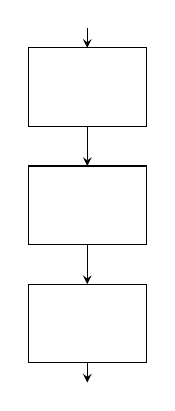
\begin{tikzpicture}
          % three boxes
          \draw (0,0) -- (1.5,0) -- (1.5,1) -- (0,1) -- (0,0);
          \draw (0,1.5) -- (1.5,1.5) -- (1.5,2.5) -- (0,2.5) -- (0,1.5);
          \draw (0,3) -- (1.5,3) -- (1.5,4) -- (0,4) -- (0,3);
          % four arrows
          \draw[-stealth] (0.75,4.25) -- (0.75,4);
          \draw[-stealth] (0.75,3) -- (0.75,2.5);
          \draw[-stealth] (0.75,1.5) -- (0.75,1);
          \draw[-stealth] (0.75,0) -- (0.75,-0.25);
        \end{tikzpicture}
        \par\vskip 4pt\ \
      \end{minipage}
      &
      \begin{minipage}{1.8in}
        \par\vskip 10pt
        \begin{tikzpicture}
          % three boxes
          \draw (1.5,0) -- (3,0) -- (3,1) -- (1.5,1) -- (1.5,0);
          \draw (0,1.75) -- (1.5,1.75) -- (1.5,2.75) -- (0,2.75) -- (0,1.75);
          \draw (3,1.75) -- (4.5,1.75) -- (4.5,2.75) -- (3,2.75) -- (3,1.75);
          % a triangle
          \draw (2.25,3) -- (3.25,3.5) -- (2.25,4) -- (1.25,3.5) -- (2.25,3);
          % and six arrows
          \draw[-stealth] (2.25,4.25) -- (2.25,4);
          \draw[-stealth] (1.25,3.5) node[above left] {\scriptsize False} -- (0.75,3.5) -- (0.75,2.75);
          \draw[-stealth] (3.25,3.5) node[above right] {\scriptsize True} -- (3.75,3.5) -- (3.75,2.75);
          \draw[-stealth] (0.75,1.75) -- (0.75,1.35) -- (2.25,1.35) -- (2.25,1);
          \draw[-stealth] (3.75,1.75) -- (3.75,1.35) -- (2.25,1.35) -- (2.25,1);
          \draw[-stealth] (2.25,0) -- (2.25,-0.25);
        \end{tikzpicture}
        \par\vskip 4pt\ \
      \end{minipage}
      &
      \begin{minipage}{1.7in}
        \centering\par\vskip 10pt
        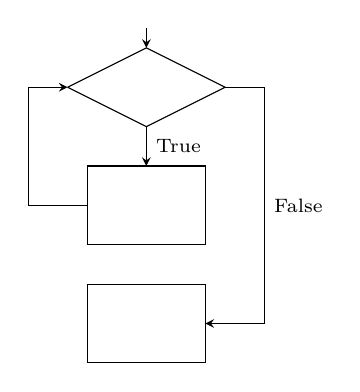
\begin{tikzpicture}
          % two rectangles
          \draw (0.25,1.5) -- (1.75,1.5) -- (1.75,2.5) -- (0.25,2.5) -- (0.25,1.5);
          \draw (0.25,0) -- (1.75,0) -- (1.75,1) -- (0.25,1) -- (0.25,0);
          % one triangle
          \draw (0,3.5) -- (1,3) -- (2,3.5) -- (1,4) -- (0,3.5);
          % five arrows
          \draw[-stealth] (1,4.25) -- (1,4);
          \draw[-stealth] (1,3) -- node[right] {\scriptsize True} (1,2.5);
          \draw[-stealth] (0.25,2) -- (-0.5,2) -- (-0.5,3.5) -- (0,3.5);
          \draw[-stealth] (2,3.5) -- (2.5,3.5) -- node[right] {\scriptsize False} (2.5,0.5) -- (1.75,0.5);
        \end{tikzpicture}
        \par\vskip 4pt\ \
      \end{minipage}
      \\
      \hline
    \end{tabular}
  \end{center}
  
  {\it\large Refer to Model 1 above as your team develops consensus answers
    to the questions below.}
    
  \quest{20 min}
      
  \Q Based only on the pictures in the model above, what do the shapes represent?
    \begin{enumerate}
      \item Rectangle
        \begin{answer}[0.4in]
          The rectangle represents a command or group of commands in a program.
        \end{answer}

      \item Diamond
        \begin{answer}[0.4in]
          The diamond represents a true/false decision that must be made.
        \end{answer}
    \end{enumerate}

  \vskip -20pt
    
  \Q Which structure best describes the types of programs you've written thus far?
    \begin{answer}[0.4in]
      The sequential structure -- our code just executes the statements in order  
    \end{answer}
    
  \Q Which structure(s) allows the programmer to create programs that decide what code to execute?
    \begin{answer}[0.4in]
      Either the branching or the looping structure.
    \end{answer}

  \newpage

  \Q A {\it relational operator} is used to test for a particular relationship between two
    values.  It returns either {\bf true}, if the relationship holds, or {\bf false}, if it 
    does not.  What relationship does each operator below test for?  If unsure, use the
    file {\tt activity05a.cpp} to try them out.
    
    \begin{enumerate}
      \itemsep 10pt
      \begin{multicols}{2}
        \item $<$  \hspace{10pt} \ans[2in]{less than}
        \item $<=$ \hspace{3pt}  \ans[2in]{less than or equal}
        \item $!=$ \hspace{5pt}  \ans[2in]{not equal}
        \item $>$  \hspace{10pt} \ans[2in]{greater than}
        \item $>=$ \hspace{3pt}  \ans[2in]{greater than or equal}
        \item $==$ \hspace{3pt}  \ans[2in]{equal to}
      \end{multicols}
    \end{enumerate}

  \vskip -30pt
    
  \Q Use the variable values below to determine the value of the
    following expressions.\key\\[-5mm]
    \begin{center}
      \begin{minipage}{3.5in}
        \begin{cpplst}
int x = 4, y = 5, z = 4;
        \end{cpplst}
      \end{minipage}
    \end{center}

    \par\vskip 10pt
    
    \begin{enumerate}
      \itemsep 10pt
      \begin{multicols}{2}
        \item \cpp{x > y}
          \hspace{14pt} \ans[0.8in]{false}
        \item \cpp{x < y}
          \hspace{14pt} \ans[0.8in]{true}
        \item \cpp{x == y}
          \hspace{9pt} \ans[0.8in]{false}
        \item \cpp{x != y}
          \hspace{10pt} \ans[0.8in]{true}
        \item \cpp{x >= z}
          \hspace{10pt} \ans[0.8in]{true}
        \item \cpp{x <= z}
          \hfill \ans[0.8in]{true}
        \item \cpp{x + y > 2 * x}
          \hfill \ans[0.8in]{true}
        \item \cpp{y * x - z != 4 \% 4 + 15}
          \hfill \ans[0.8in]{false}
        \item \cpp{pow(x,2) == abs(-16)}
          \hfill \ans[0.8in]{true}
      \end{multicols}
    \end{enumerate}

    \vskip -20pt
 
  \Q What are the two possible answers for each expression in that last question?
    \begin{answer}[0.5in]
      They can be true or false.
    \end{answer}
          
  \Q Assume the following strings have been defined. Determine the results of the following
    expressions.
    \begin{center}
      \begin{minipage}{3.5in}
        \begin{cpplst}
string word1 = "hello";
string word2 = "good-bye";
        \end{cpplst}
      \end{minipage}
    \end{center}

    \par\vskip 10pt
    
    \begin{enumerate}
      \itemsep 10pt
      \begin{multicols}{2}
        \item \cpp{word1 == word2}
          \hspace{14pt} \ans[1in]{false}
        \item \cpp{word1 != word2}
          \hspace{14pt} \ans[1in]{true}
        \item \cpp{word1 < word2}
          \hspace{14pt} \ans[1in]{false}
        \item \cpp{word1 >= word2}
          \hspace{14pt} \ans[1in]{true}
      \end{multicols}
    \end{enumerate}

  \Q How do relational operators work on strings?
    \begin{answer}[1in]
      \par
      They compare strings lexicographical.  Meaning, words that come first in the dictionary would be
      smaller than others.  To be equal, the strings must be identical.
    \end{answer}
